\newaufgabe{
Zum CBC Betriebsmodus von Blockciphern: Erklären sie, (i) warum die angegebene
Entschlüsselungsformel tatsächlich funktioniert, (ii) wie es zu den beschriebenen
Plaintextfehlern nach dem Auftreten eines 1-Bit Ciphertextfehler kommt und (iii)
warum CBC self-recovering ist.
}
\begin{proof}
    Zu (i): Die Entschlüsselungsformel für den CBC Modus ist korrekt.
    \begin{align*}
        P_i &=C_{i-1}\oplus D_k(C_i)\\
            &=C_{i-1}\oplus D_k(E_k(P_i\oplus C_{i-1}))\\
            &=C_{i-1}\oplus P_i\oplus C_{i-1}&&\mid \text{XOR Rechenregeln}\\
            &=P_i
    \end{align*}    
\end{proof}
\begin{figure}[h]
    \centering
    \begin{subfigure}[b]{0.4\textwidth}
        \centering
        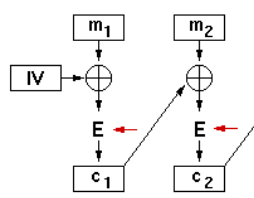
\includegraphics[width=\textwidth]{img/encryption.png}
        \caption{Verschlüsselung}
        \label{fig:cbc_enc}
    \end{subfigure}
    \hfill
    \begin{subfigure}[b]{0.4\textwidth}
        \centering
        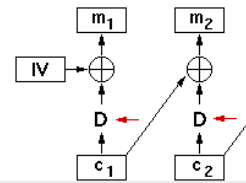
\includegraphics[width=\textwidth]{img/decryption.png}
        \caption{Entschlüsselung}
        \label{fig:cbc_dec}
    \end{subfigure}
    \caption{CBC Verschlüsselung \& Entschlüsselung (Ausschnitt)}
    \label{fig:cbc}
\end{figure}
Zu (ii): Angenommen es ist bei einem beliebigen (aber fixen) $C_i$ ein 1-Bit Fehler
aufgetreten. Dann wird bei der Entschlüsselung nicht mehr $C_i$ sondern ein 
geändertes $C_i'$ entschlüsselt (siehe Abb.\ref{fig:cbc_dec}). Durch den 
\textit{Lawineneffekt} ensteht ein ganz anderer Plaintext und der gesamte 
Block ist "`zerstört"'. Der nächste Block $C_{i+1}$ wird nun zuerst entschlüsselt
und anschließend mit $C_{i}'$ geXORed. $C_{i}'$ unterscheidet sich aber nur
durch ein einzelnes Bit von dem ursprünglich zur verschlüsselung verwendeten 
$C_i$. Also wird sich auch genau 1-Bit nach der XOR-Verknüpfung in $P_{i+1}$ 
falsch sein.\vspace*{1em}\newline
Zu(iii): CBC ist self-recovering da der fehlerhafte Cipherblock nur zur Entschlüsselung
des direkt darauffolgenden verwendet wird. Der übernächste Block verwendet den fehlerhaften
Block nicht mehr, also pflanzt sich der Fehler auch nicht weiter fort.